
\begin{figure*}[t]
	\includegraphics[width=7in]{sccPipelines.png}
	\caption{SCC directed acyclic graphs for each of the applications. \hl{Update}}
	\label{fig:sccPipelines}
\end{figure*}

\section{Prototype}
\label{sec:prototype}

This section describes our prototype.  We developed six
applications to run on the mobile device and a set of 
sensor data processing algorithms to run on the sensor
node.  Using these algorithms, we constructed a SCC for
each of the applications.  To evaluate the applications 
and the simple classifiers, we developed a trace-driven
simulator.  The simulator uses power measurements 
collected from a Nexus 4 based hardware implementation
to estimate average power consumption for a given trace
and sensing configuration.

\subsection{Applications}

\subsubsection{Accelerometer Applications}

We developed three applications that detect activities that the robot
can perform: walking, posture transitions, and headbutts.  
We chose these
actions because they have similar acceleration signatures to human
activities.  A walking robot has a similar acceleration signature as
its human counterpart, though at a lower intensity.  The headbutts are
meant to represent very infrequent human actions such as falling.  We
found that robot stance transitions between the normal and sitting
postures are very similar in their acceleration signature to humans
sitting down and standing up.  In Section~\ref{sec:results} we show
that the energy saving measured in our experiments with the robot
approximate closely the results of experiments conducted on limited
traces collected from human subjects.

{\bf Steps} Counts how many steps the robot takes when it
  walks. The algorithm is based on the human step detection algorithm
  proposed by Ryan Libby in~\cite{libbyFootstepDetection}. The
  application takes in raw accelerometer readings and applies a
  low-pass filter on the x-axis acceleration. It then searches for
  local maxima in the filtered x-axis acceleration. Local maxima
  between $2.5\:m/s^2$ and $4.5\:m/s^2$ are detected as steps, given
  that no other steps were detected within the last 100 ms.

{\bf Transitions} Detects transitions between sitting and
  standing.  The application monitors changes in acceleration due to
  gravity on the y and z axes to determine the orientation of the
  device. If the z-axis (up-down relative to the dog) acceleration is
  between $9 m/s^2$ and $11 m/s^2$, and the acceleration on the y-axis
  (front-back relative to the dog) is between $-1 m/s^2$ and $1
  m/s^2$, the device is in a horizontal position and the robot is
  assumed to be in a standing posture. Similarly, if the z-axis
  acceleration is between $7.5 m/s^2$ and $9.5 m/s^2$, and the
  acceleration on the y-axis is between $3.5 m/s^2$ and $5.5 m/s^2$,
  the device is in an angled position and the robot is assumed to be
  in a sitting posture. The application detects transitions by looking
  for posture changes.

{\bf Headbutts} Detects a sudden forward head movement.  The
  application monitors the y-axis acceleration and searches for local
  minima between $-3.75\:m/s^2$ and $-6.75\:m/s^2$.

\subsubsection{Audio Applications}

{\bf Siren Detector} Detects sirens originating from
emergency vehicles.  The application applies a 750 Hz high-pass filter 
in order to remove a significant
potion of sounds that aren't sirens.  The data in each window is transformed 
to the frequency domain using a FFT in order to extract the magnitude of the 
dominant frequency and the mean magnitude of all frequency bins.  The ratio
of the dominant frequency magnitude and the mean magnitude is used to determine
if the window contains pitched sounds.  Pitched sounds between 850 Hz and 1800 Hz
that last longer 650 ms are classified as sirens. 

{\bf Music Journal} Creates a list of all the songs heard during the
day using the web services provided by Echoprint.me~\cite{echoprint}.

{\bf Phrase Detection} Detects specific phrases using web services
accessible via the Google Speech API.


\subsection{Sensor Data Processing Algorithms}
\label{sec:sensorDataAlgorithms}


We implemented the following processing algorithms:

\begin{itemize}

	\item {\bf Windowing} Partitioning sensor data into rectangular or Hamming windows.
		
	\item {\bf Transform} Fast Fourier Transform (FFT) from time-domain to frequency-domain.
	  
	\item {\bf Data Filtering} 
		\begin{itemize}
			\item Noise-reduction algorithm based on exponential moving average with 
	  configurable degree of weighting decrease.
			\item FFT-based low-pass filtering.
			\item FFT-based high-pass filtering.
		\end{itemize}

	\item {\bf Feature Extraction} 
		\begin{itemize}
			\item Magnitude of acceleration vector computation.
			\item Zero Crossing Rate computation.
			\item A set of statistical functions.
			\item Determination of magnitude of dominant frequency.
		\end{itemize}

	\item {\bf Admission Control} Configurable high or low thresholds on values of extracted features.
  
\end{itemize}


\subsection{Simple Configurable Classifiers}
\label{sec:classifiers}

\iffalse
\begin{figure*}[t]
{\small
	\begin{verbatim}
# segment audio data
$DATA > window type=rect size=256000 overlap=32000 > $win

# compute variance of amplitude
$win > stat type=var > $varamp

# compute variance of zero crossing rate
$win > window type=rect size=500 | extract type=zcr | stat type=var > $varzcr

# perform threshold-based admission control
$varamp > admissioncontrol type=threshold min=0.002 max=0.013 > $acamp
$varzcr > admissioncontrol type=threshold min=150 max=1100 > $aczcr

# check if admission control passed
assert $acamp
assert $aczcr

# pass raw sensor data to application
return $win
	\end{verbatim}
}
	\caption{SCC definition for music detection}
    \label{fig:sccLanguageMusicDetectionOld}
\end{figure*}
\fi

\begin{figure*}[t]
{\small
	\begin{verbatim}
# feature extraction: variance of amplitude 
$VARAMP = Aggregate(type=var, size=256000, advance=32000)

# feature extraction: zero-crossing rate 
$ZCR = Aggregate(type=zcr, size=500)

# feature extraction: variance of zero-crossing rate 
$VARZCR = Aggregate(type=var, size=64)

# threshold-based admission control to be applied to the extracted zero-crossing rate
$AC = AdmissionControl(type=threshold, min=100, max=200)

# threshold-based admission controls
$AMP_AC = AdmissionControl(type=threshold, min=0.002, max=0.013)
$ZCR_AC = AdmissionControl(type=threshold, min=150, max=1100)

# Define data stream flows
$DATA >        $VARAMP > $AMP_AC
$DATA > $ZCR > $VARZCR > $ZCR_AC

Assert($AMP_AC)
Assert($ZCR_AC)
	\end{verbatim}
}
	\caption{SCC definition for music detection}
    \label{fig:sccLanguageMusicDetectionOld}
\end{figure*}

We created a simple classifier for each of the six applications using
the processing algorithms described in section~\ref{sec:sensorDataAlgorithms}. 
Figure~\ref{fig:sccPipelines} shows the directed acyclic graph representation
for each of the SCC we constructed.  Generally, the simple classifiers are 
simplified versions of the detection algorithms implemented by the
applications.  However, specific
phrase detection is a complex process that requires algorithms not implemented
by prototype.  As a compromise, the SCC for the phrase detection application
is used to wake-up the device when any speech is detected.

Each of the classifiers ends with an admission control step with configurable 
thresholds.  A classifier detects events of interest when the relevant
data or extracted features fulfil the admission control conditions.  

Figure~\ref{fig:sccLanguageMusicDetection} shows the definition of SCC
for the music detection application.  


\subsection{Trace-driven Simulator}

We created a trace-driven simulator in order to evaluate 
the performance of the applications and their simple 
classifiers.  The simulator has the following inputs and
outputs:
\begin{itemize}
	\item Inputs:
		\begin{itemize}
			\item A file containing the sensor data.
			\item A file containing ground truth information.
			\item A sensing configuration (see Section~\ref{sec:configurations})
		\end{itemize}
		
	\item Outputs:
		\begin{itemize}
			\item Amount of time that device would be awake and asleep.
			\item Number of wake-ups.
			\item Event of interest precision and recall.
		\end{itemize}
\end{itemize}

For the accelerometer applications we also created a hardware
implementation described in detail in the following section.

Using real power measurements from our hardware implementation,
we created a model to estimate power consumption based on the
outputs from the simulator. 

\subsection{Prototype Implementation}

\begin{figure}[t]
	\centering
	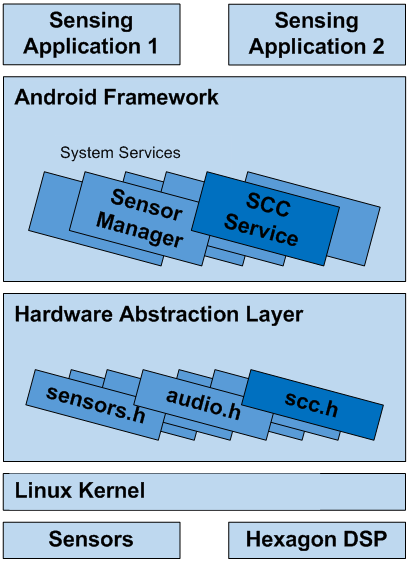
\includegraphics[width=3.1in]{dragonboardPrototype.png}
	\caption{Prototype architecture.}
    \label{fig:dragonboardPrototype}
\end{figure}

We implemented a prototype of our system using a DragonBoard 8094 
Development Kit.  The low-power sensor node is implemented using
the Hexagon DSP that comes bundled with the Snapdragon 810 CPU.  Figure
\ref{fig:dragonboardPrototype} shows a high-level diagram of the
prototype's architecture.

Unfortunately, we were unable to use the Android's SensorManager and
the Hardware Abstraction Layer's sensor interface for our purposes
because they do not allow applications to pass any data down to the
sensors.  Since interested applications need to pass a 
representations of their SCC to the sensor node, the SensorManager
would need to be augmented with the necessary functions and the 
HAL's sensor interface would need to be modified.  Alternatively,
we chose to create a dedicated interface for SCC in the HAL and
add a system service to expose the SCC features to the applications.

\hl{TODO: explain communication with the sensor node (Hexagon DSP or microcontroller)}

\hl{TODO: explain how the sensor-node implementation can be easily swapped}

\bgroup
\def\arraystretch{1.5}
\begin{table*}[t]
\centering
{\small
	\begin{tabular}{| l | c | c |}
		\hline
		\textbf{Main CPU State}						& \textbf{Hexagon DSP State}	& \textbf{Average Power Consumption (mW)} 	\\ \hline
		Awake, running sensor-driven application  	& Asleep						& xxx 										\\ \hline
		Asleep										& Awake, running a SCC			& xxx 										\\ \hline
		Asleep 										& Asleep						& xxx 										\\ \hline \hline
		
		\textbf{Main CPU Transition}				& \textbf{Average Power Consumption (mW)} 		& \textbf{Average Duration} \\ \hline
		Asleep-to-Awake 							& xxx 											& x second \\ \hline
		Awake-to-Asleep 							& xxx 											& x second \\ \hline
	\end{tabular}
}
	\caption{DragonBoard 8094 Development Kit Power Profile}
	\label{table:powerProfileDragonboard}
\end{table*}
\egroup

We power profiled the prototype implementation.  The results are summarized in
Table~\ref{table:powerProfileDragonboard}.  During all the measurements, the
device's screen, WiFi and GPS were turned off \hl{TODO: update}.  While the device is
sleeping, its power usage is very low, consuming only xxx mW.  While
awake, the power consumption is significantly higher, averaging xxx
mW.  During our power measurements we noticed that additional energy is
consumed during transitions between the asleep and awake states.  Each
transition takes about xxx second.  During a wake-up transition, the
average power consumption goes up to xxx mW, while during an
awake-to-asleep transition the average power consumption is xxx mW.

\iffalse
\subsection{Hardware Implementation Old}

\begin{figure}[t]
	\centering
	\includegraphics[width=3.1in]{prototype_architecture.png}
	\caption{Prototype architecture.}
    \label{fig:prototypeArchitecture}
\end{figure}

We implemented a prototype of our system using a Google Nexus 4 phone
running Android 4.2.2.  The low-power sensor node is implemented using
a Texas Instruments micro-controller board attached to an
accelerometer sensor.  We chose to focus our efforts on the
accelerometer sensor because of its relative simplicity and the
availability of a wide range of accelerometer-based applications on
various mobile application markets.  Figure
\ref{fig:prototypeArchitecture} shows a high-level diagram of the
prototype's architecture.

The Nexus 4 and TI board communicate over the UART port made available
by the Nexus 4 debugging interface via the physical port used by the
audio interface.  The serial connection provides sufficient bandwidth
to support low bit-rate sensors, such as the accelerometer, a
microphone or GPS.  However, extending the prototype to work with
higher bit-rate sensors like the camera would require a higher
bandwidth data bus, such as $I^2C$.

This section describes our extensions to the phone and the
sensor node implementation.

\subsubsection{Nexus 4}
\label{subsec:nexus}

On the Nexus phone we extended Android's SensorManager to include the
new features made available by our system. To prevent a steep learning
curve, our goal was to provide an API very similar to Android's
existing sensors API.  

We extended the Sensor Manager to allow developers to define SCC by building
a pipeline of pre-defined data processing algorithms and configuring their
parameters. The available types of processing algorithms are
described in Subsection~\ref{sec:sensorDataAlgorithms}.

We also created a UART stub to facilitate communication between the
mobile phone and the sensor node. The UART stub is called when
the sensor node detects an event based on its SCC.
In turn, the UART stub is a shell script that notifies the
SensorManager using an Android Intent~\cite{androidintents}.

For our prototype we avoided modifying the Android kernel in any way.
Because the current prototype uses the UART port for communication
with the sensor node, we were able to constrain our implementation to
the user space.  An integrated implementation would likely make use of
a higher bandwidth bus such as the $I^2C$ bus and require a custom
driver.

\bgroup
\def\arraystretch{1.5}
\begin{table*}[t]
\centering
{\small
	\begin{tabular}{| l | c | c |}
		\hline
		\textbf{State}								& \textbf{Average Power Consumption (mW)} 		& \textbf{Average Duration} \\ \hline
		Awake, running sensor-driven application 	& 323 											& N/A \\ \hline
		Asleep 										& 9.7 											& N/A \\ \hline
		Asleep-to-Awake Transition 					& 384 											& 1 second \\ \hline
		Awake-to-Asleep Transition 					& 341 											& 1 second \\ \hline
	\end{tabular}
}
	\caption{Google Nexus 4 power profile.}
	\label{table:powerProfileNexus}
\end{table*}
\egroup

We power profiled the Google Nexus 4.  The results are summarized in
Table~\ref{table:powerProfileNexus}.  During all the measurements, the
device's screen, WiFi and GPS were turned off.  While the device is
sleeping, its power usage is very low, consuming only 9.7 mW.  While
awake, the power consumption is significantly higher, averaging 323
mW.  During our power measurements we noticed that additional energy is
consumed during transitions between the asleep and awake states.  Each
transition takes about 1 second.  During a wake-up transition, the
average power consumption goes up to 384 mW, while during an
awake-to-asleep transition the average power consumption is 341 mW.


\subsubsection{Sensor Node}
\label{subsec:sensorNode}

The low-power sensor node consists of a driver that talks to
the accelerometer sensor, a set of data processing algorithms, a controller,
and an UART driver for communicating with the phone.  The controller
orchestrates the execution of the algorithms, and uses the UART driver to
wake up the phone when an event is detected by the SCC.  The UART driver
opens a serial port and then uses a TTY to copy the sensor readings
and starts the shell script that notifies the Sensor Manager.


\subsubsection{Hardware Options}

We evaluated two low-power micro-controllers manufactured by Texas
Instruments, the MSP430 and the Stellaris LM4F\-120H5QR.  The MSP430 has
the advantage of requiring very little power, consuming only 3.6 mW
while awake.  However, it has limited memory and cannot perform complex
analysis of sensor data in real-time.  In our tests, it was unable to
run the algorithms based on Fast Fourier Transforms in real-time.  
The Stellaris LM4F120H5QR is powered by a Cortex-M4 processor.  It can 
batch a higher number of accelerometer
readings and can run all our algorithms in real-time.  However, this
micro-controller has an energy footprint an order of magnitude greater
than the MSP430, consuming an average of 49.4 mW while awake.

\begin{figure}[t]
	\centering
	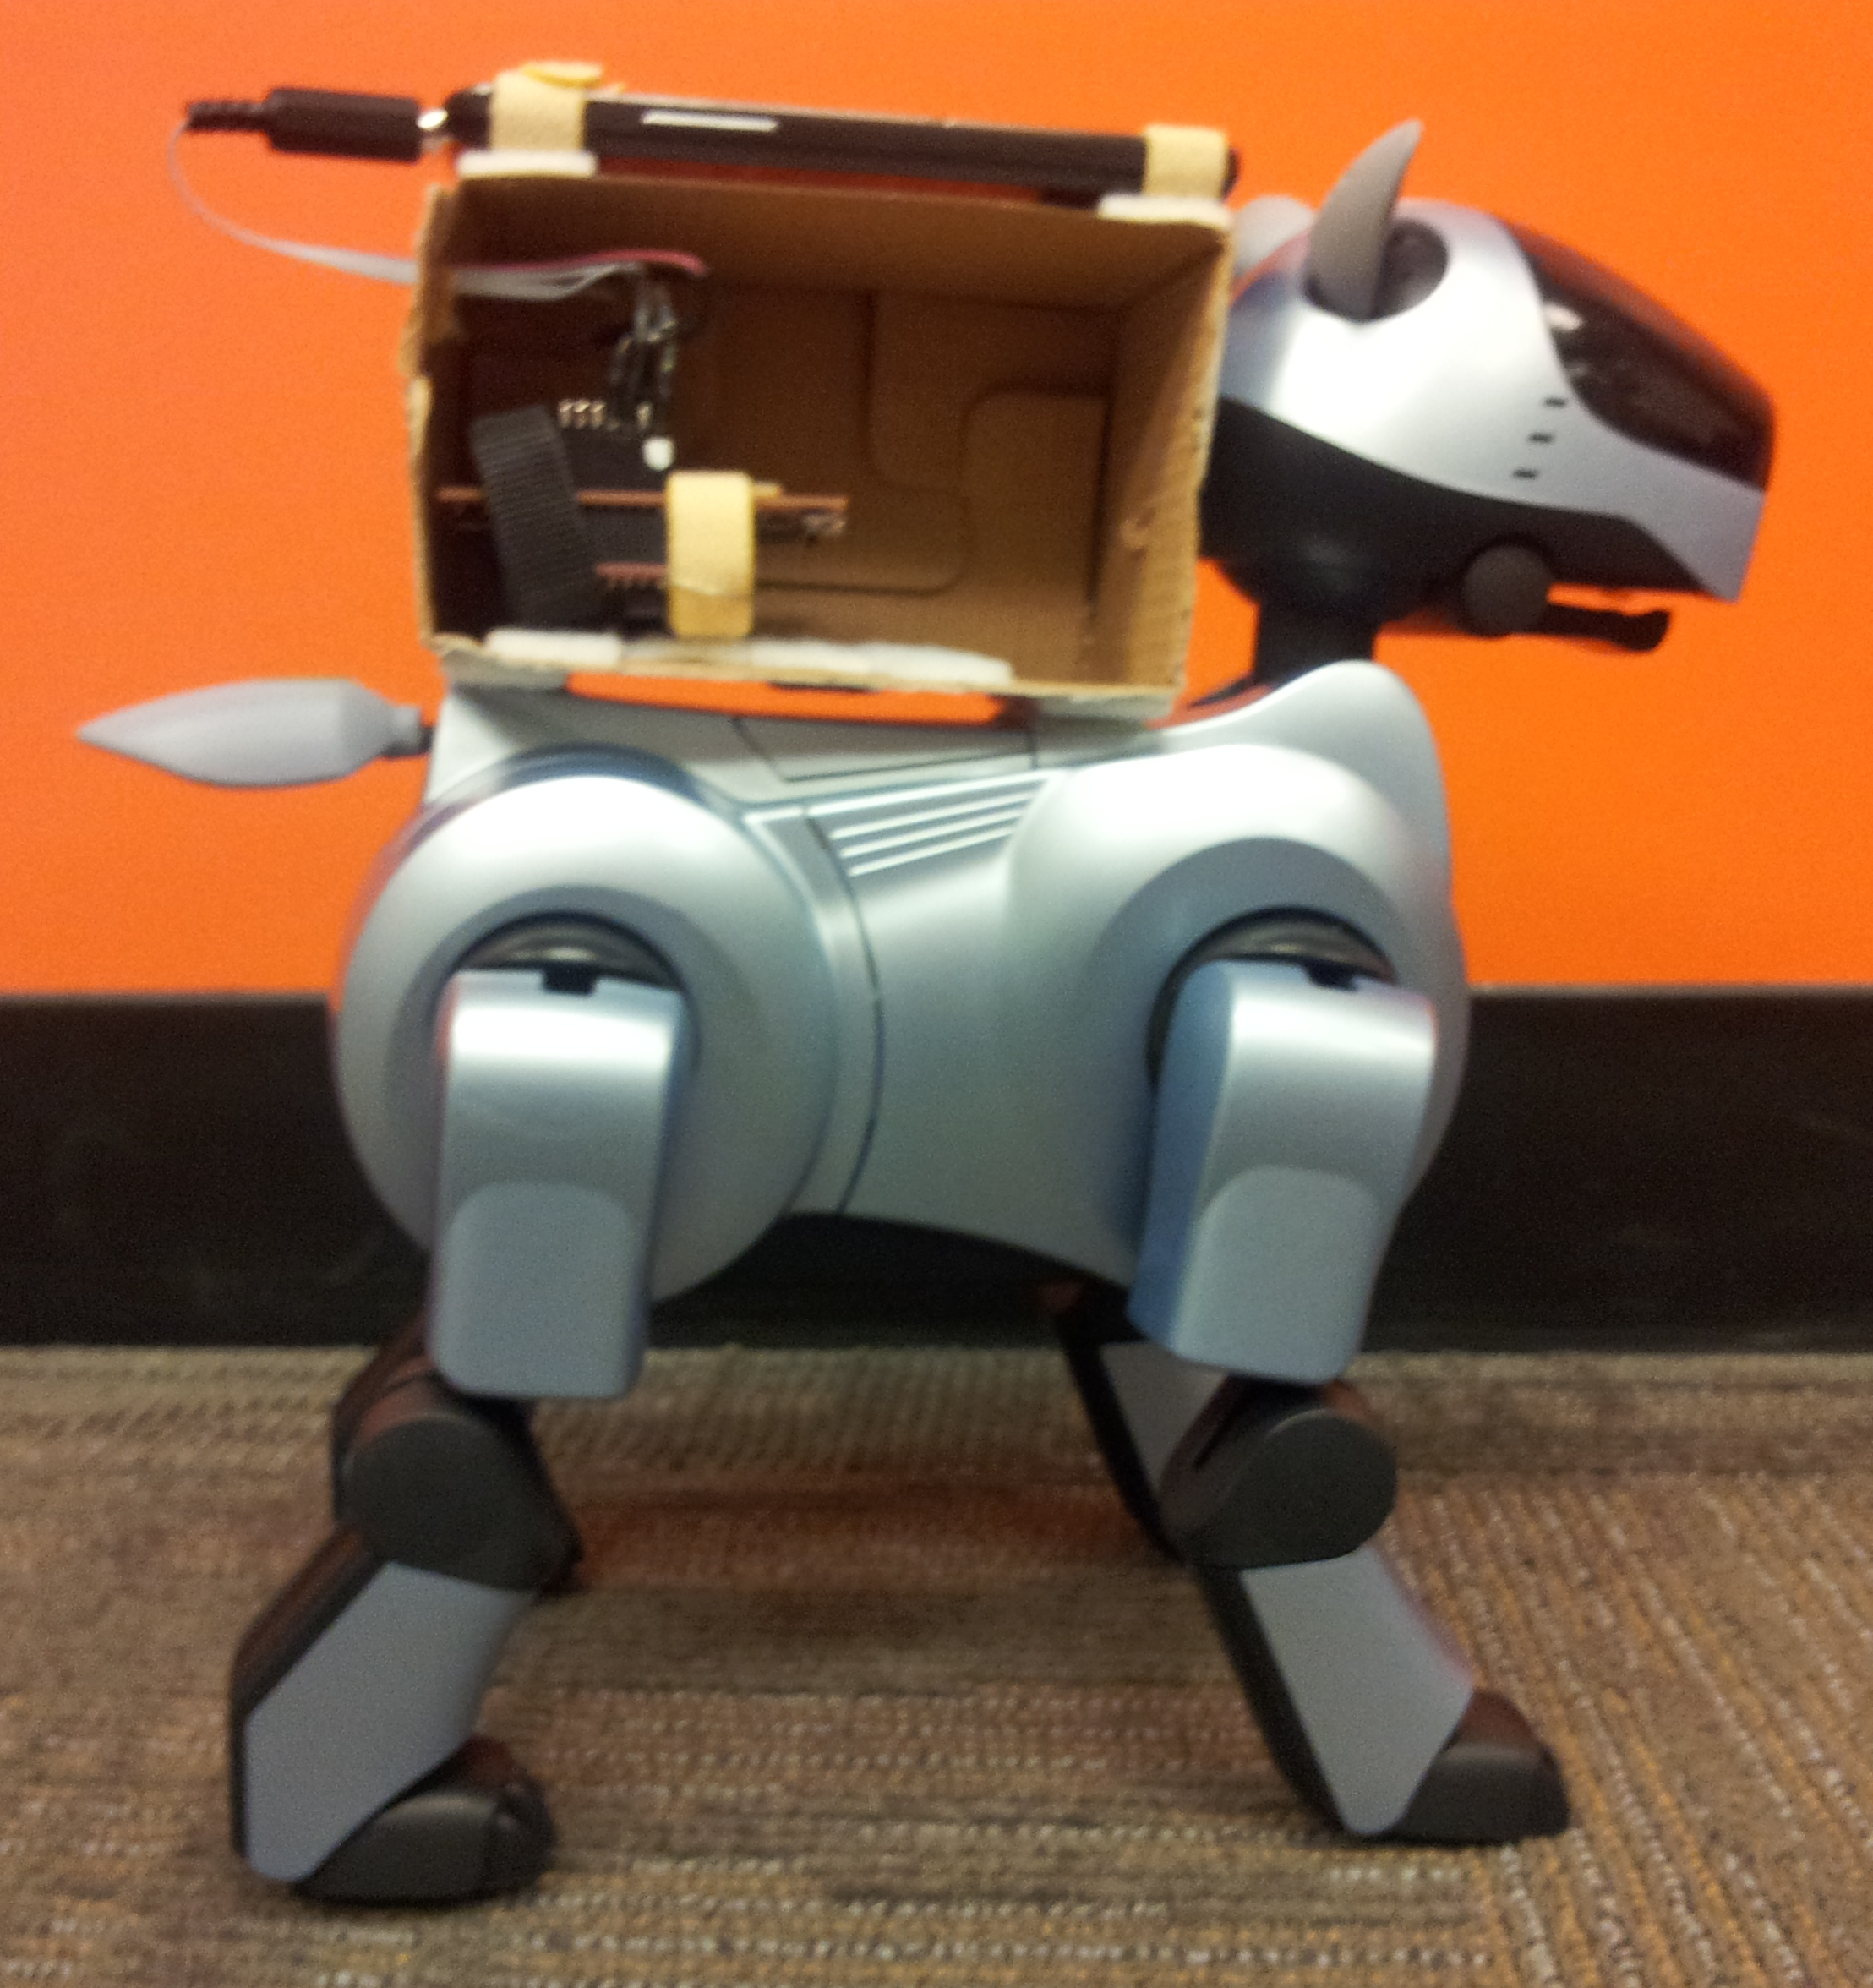
\includegraphics[width=3in]{aibo_ers_210.jpg}
	\caption{AIBO ERS 210 with Smartsensor prototype.}
	\label{fig:aibo}
\end{figure}

\fi
